\makeatletter
\def\input@path{{../../}}
\makeatother
\documentclass[../../main.tex]{subfiles}

\graphicspath{
	{../../img/}
	{../img/}
	{img/}
}

\begin{document}
	
	
	\subsection{Вычисление объемов с помощью ПовИ}
	Поскольку объем $V$ может быть найден по формуле:
	
	\[ V = \iiint \limits_W dx dy dz \]
	
	То если в формуле Остроградского-Гаусса подынтегральная функция тождественно равна 1, то имеем:
	
	\[ V = \iint \limits_{\Pi} Pdydz+Qdzdz+Rdxdy = * \]
	
	Это будет выполнятся например для:
	
	\[ *=  \iint \limits_{\Pi} x \; dydz = \iint \limits_{\Pi} y \; dxdz = \iint \limits_{\Pi} z \; dxdy = \iint \limits_{\Pi}  \frac{1}{3} x \; dydz + \frac{1}{3} y \; dxdz + \frac{1}{3} z \; dxdy \]
	
	Рассмотрим пример:
	
	\begin{example}
	
	Найти объем тела ограниченного поверхностью, которая задается формулой:
	
	\[ \Pi:\begin{cases} x=\left( b + a \cos{v} \right) \cos{u} \\ 
	y = \left( b + a \cos{v} \right) \sin{u} \\ 
	z= a \sin{v} \\
	- \pi \leq v \leq \pi \\
	0 \leq u \leq 2\pi	
	\end{cases} \]	
	С ограничением $0 < a < b$. Это тело представляет собой Тор:
	
	
	\begin{center}
		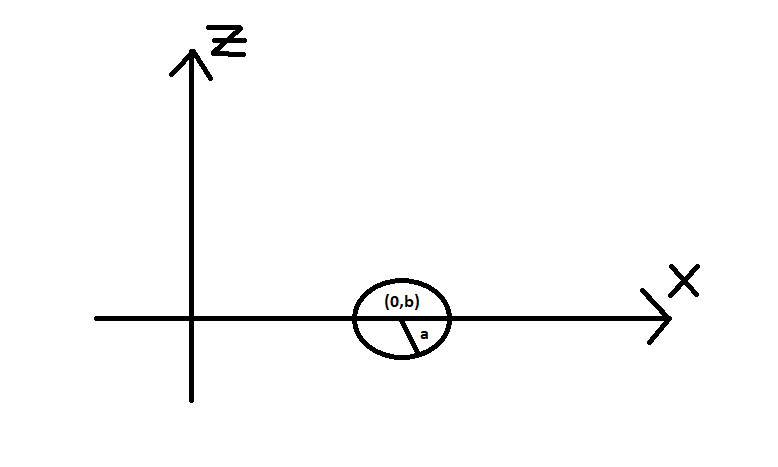
\includegraphics[scale = 0.8]{lec_25_Thor_POVI}
	\end{center}
	Получаем тело вращения вокруг оси $Oz$.
	
	Воспользуемся формулой:
	
	\[ V = \iint \limits_{\Pi} zdxdy = \int_{0}^{2\pi}du \int_{-\pi}^{\pi}z\left( u,v \right) \; C \; dudv \] 
	
	Где:
	
	\[ C = \begin{vmatrix}
	x_u' & y_u' \\
	x_v' & y_v' \\
	\end{vmatrix} = x_u'  y_v' - x_v'  y_u' = a \sin^2{u} \sin{v} \left( b + a\cos{v} \right) + a \cos^2{u} \sin{v} \left( b + a\cos{v} \right)  = a \left( b + a\cos{v} \right) \sin{v}  \]
	
	Тогда: 
	
	\[ V = a^2 \int_{0}^{2\pi} du \int_{-\pi}^{\pi} \sin^2{v} \left( b + a\cos{v} \right) \; dv = 2\pi a^2 \left(  a \int_{-\pi}^{\pi } \sin^2{v} \cos{v} \; dv + b \int_{-\pi}^{\pi } \frac{1-\cos{2v}}{2} \; dv  \right) = 2\pi^2  \]
	\end{example}

	\section{Формула Стокса}
	
	Пусть есть поверхность $\Pi$ ограниченная кривой $l$. Говорят, что направление обхода границы $l$ согласовано с выбором поверхность $\Pi$, если при движении в таком направлении $\Pi$ остается слева, а вектор нормали к $\Pi$ направлен снизу вверх к наблюдателю.
	
	\begin{center}
		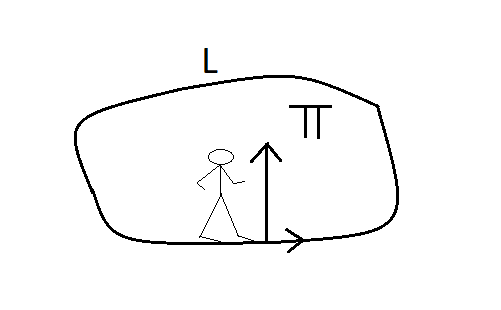
\includegraphics[scale = 0.8]{lec_25_Human_direction}
	\end{center}
	
	Будем предполагать, что в дальнейшем такое согласование есть.
	
	\begin{theorem}
		Пусть функции $P,Q,R$ непрерывны и имеют непрерывные частные производные в области $D$. Тогда:
		
		\[ \oint \limits_L P \; dx + Q \; dy + R \; dz = \iint \limits_{\Pi} \left( Q_x' - P_y'\right)dxdy + \left( R_y' - Q_z'\right)dydz + \left( P_z' - R_x'\right)dzdx     \]
		
		Справедлива формула выше, которую называют формулой Стокса.
		
		Как ее запомнить?
		
		\begin{center}
			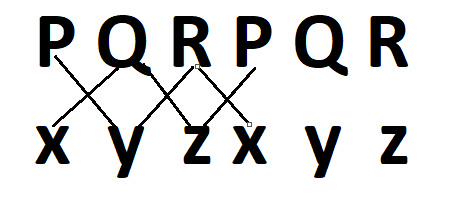
\includegraphics[scale = 0.6]{lec_25_PQR}
		\end{center}
		
		\begin{proof}
			Пусть $\Pi$ задана уравнениями:
			
			\[ \Pi : \begin{cases} 
			x = x\left( u,v\right) \\ 
			y = u\left( u,v\right) \\ 
			z = z\left( u,v\right)  
			\end{cases} \]
			Где $\left( u,v \right) \in \Delta \subset \mathbb{R}^2$ и $\lambda$-граница области $\Delta$.
			
			\[ \lambda : \begin{cases} 
			u = u \left( t \right)  \\ 
			v = v \left( t \right) \\ 
			t \in T \subset \mathbb{R}  
			\end{cases} \]
			
			Совершенно понятно, что если мы возьмем точки на $\lambda$, то получим точки на $\Pi$. Возьмем произвольное $t$, тогда точка:
			
			 \begin{gather*} x = x\left( u\left( t\right), v\left( t\right)   \right) \\
			 y = y\left( u\left( t\right), v\left( t\right)   \right) \\
			 z = z\left( u\left( t\right), v\left( t\right)   \right) \\
			 \end{gather*}
			 
			 Принадлежит $l$\--- границе $\Pi$
			 
			 Рассмотрим переход к 1И:
			 
			 \[ \oint \limits_L P\left( x,y,z \right) \; dx = \int \limits_T P \left( x\left( u\left( t\right), v\left( t\right)   \right), y\left( u\left( t\right), v\left( t\right)   \right)  ,z\left( u\left( t\right), v\left( t\right)   \right) \right) \left( x_u' u_t' + x_v' u_t' \right) \; dt = *  \]
			 
			 Перейдем к КрИ по кривой по кривой $\lambda$:
			 
			 \[ * = \int \limits_{\lambda} P\left( x,y,z \right) \; dx = \int \limits_T P \left( x\left( u\left( t\right), v\left( t\right)   \right), y\left( u\left( t\right), v\left( t\right)   \right)  ,z\left( u\left( t\right), v\left( t\right)   \right) \right) \left( x_u' \; du + x_v ' \; dv \right) =  \]
			 
			 \[ = \int \limits_{\lambda} P x_u' \; du + \int \limits_{\lambda} P x_v' \; dv =  \left[   \text{Применим формулу Грина}  \right] =   \]
			 
			 \[ = \iint \limits_{\Delta} \left( \frac{\partial}{\partial{v}} P x_v' - \frac{\partial}{\partial{u}} P x_u' \right) \; du dv = \iint \limits_{\Delta} \left(
			 P_u' x_v ' + P x_{vu} '' - P_v' x_u' - P x_{uv}'' \right) \; du dv  =  \]
			 
			 \[ \iint \limits_{\Delta} \left( \left( P_x' x_u' + P_y' y_u' + P_z ' z_u' \right) x_v' - \left( P_x' x_v' + P_y' y_v' + P_z ' z_v' \right) x_u'  \right) \; du dv =  \]
			
			\[ = \iint \limits_{\Delta} \left( P_y'\left( y_u' x_v' - y_v' x_u' \right) + P_z'\left( z_u' x_v' - z_v' x_u' \right)   \right) \; du dv = \iint \limits_{\Delta} \left( P_y' \begin{vmatrix} x_u' & y_u' \\ x_v' & y_v'  \end{vmatrix} + P_z' \begin{vmatrix} z_u' & x_u' \\ z_v' & x_v'  \end{vmatrix} \right) \; dudv =      \]
			
			\[ = \iint \limits_{\Delta}  \left( P_z' B - P_y' C  \right) \; dudv = \iint \limits_{\Pi}  P_z' \; dxdz - P_y' dxdy     \]
			
			Аналогично рассуждая, получаем:
			
			 \begin{equation} \label{P_oints_Stocks} \oint \limits_L P \; dx = \iint \limits_{\Pi}  P_z' \; dxdz - P_y' dxdy \end{equation}\\
			\begin{equation}  \label{Q_oints_Stocks} \oint \limits_L Q \; dy = \iint \limits_{\Pi}  Q_x' \; dxdy - Q_z' dydy \end{equation}\\
			\begin{equation}  \label{R_oints_Stocks} \oint \limits_L R \; dz = \iint \limits_{\Pi}  R_y' \; dydz - R_x' dzdx \end{equation}
			
			Складывая \eqref{P_oints_Stocks},\eqref{Q_oints_Stocks},\eqref{R_oints_Stocks}, получаем формулу Стокса.
			 
		\end{proof}	
	\end{theorem}
			
			
			\begin{example}
				\[ I = \int \limits_L \left( y-z \right) dx + \left( z-x \right) dy + \left( x-y \right) dz  \]
				
				\[ L: \begin{cases}
					x^2 + y^2 = a^2 \bigcap \frac{x}{a} + \frac{z}{h} = 1 \\
					h,a > 0 
				   \end{cases}
				 \]
				
		
			Уточним, что $L$ пробегается так, что если смотреть с положительной стороны $Ox$, то движение против часовой стрелки.
			
			%{\Huge \bf ТУТ ЦИЛИНДР КРЧ ИЗ ПРИМЕРА}
			
			Сечением будет эллипс, у которого одна ось равна $2a$, а вторая $2b$, т.е. полуоси \--- $a, \sqrt{a^2 + h^2} = b$. Воспользуемся формулой Стокса и в качестве $\Pi$ возьмем плоскость с вектором нормали:
			
			\[ \vec{N}\left( \frac{1}{a}, 0 , \frac{1}{h} \right)  \]
			
			его длина:
			
			\[ \left| \vec{N} \right|= \sqrt{\frac{1}{a^2} + \frac{1}{h^2} } = \frac{\sqrt{a^2 + h^2}}{ah}  \]
			
			и его направляющие косинусы:
			
			\[ \vec{n} = \left( \frac{h}{\sqrt{a^2 + h^2}}, 0, \frac{a}{\sqrt{a^2 + h^2}} \right)      \]
			
			Тогда по формуле Стокса:
			
			\[ I = \iint \limits_{\Pi} -2 \; dxdy - -2 \; dydz - -2 \; dzdx = \left[ \text{Перейдем от ПовИ-2 к ПовИ-1 } \right] = -2 \iint \limits_{\Pi} \frac{h+a}{\sqrt{a^2 + h^2}}  \; ds =        \]
			
			\[ = -2\frac{a+h}{\sqrt{a^2 + h^2}}  S_{\text{эллипса}} = -2\frac{a+h}{\sqrt{a^2 + h^2}} \pi a \sqrt{a^2 + h^2} = -2 \pi a \left( a+h \right)       \]
			
		\end{example}
			
		\section{Основная Теорема о КРИ в пространстве}
		
		Говорят, что область $D \subset \R ^3$	поверхностно односвязная, если на любой замкнутый контур $l \subset D$ можно натянуть поверхность лежащую в $D$.
		
		\begin{theorem}
			Пусть в поверхностно-односвязной области $D$ заданы функции $P,Q,R$ непрерывные и имеющие частные производные 1 порядка. Следующие условия равносильны:
			
			
			
			\begin{enumerate}
				\item $\forall L \subset D \oint \limits_L P \; dx + Q \; dy + R \; dz = 0 $
				\item $ \int \limits_{{\tiny \overbow{AB}}} P \; dx  Q \; dy + R \; dz \;\; $ не зависит от пути интегрирования
				\item выражение $P\;dx + Q\;dy+R\;dz$ является полным дифференциалом, т.~е. 
				\[ \exists F \; | \; dF = P\;dx + Q\;dy+R\;dz \]
				\item В $D$ выполнены условия Эйлера:
				\[ Q_x' = P_y', \; Q_z' = R_y', \; P_z' = R_x'  \]
			\end{enumerate}
		\begin{proof}
			Доказательство аналогично доказательству аналогичной теоремы для $\R ^2$
		\end{proof}	
			
		\end{theorem}
		
		Функция $F = F\left( x,y,z\right) $ может быть найдена например по формуле ниже в некоторых простейших случаях:
		
		\[ F\left( x,y,z\right) = \int_{x_0}^{x} P\left(x,y,z \right)dx + \int_{y_0}^{y} Q\left(x_0,y,z \right)dy + \int_{z_0}^{z} R\left(x_0,y_0,z \right)dz \]
		
		Где $\left( x_0,y_0,z_0\right) $\--- произвольная фиксированная точка из $D$ 
	
	\end{document}
